\documentclass[a4paper,10pt]{article}
\usepackage[utf8]{inputenc}
\usepackage[T1]{fontenc}
\usepackage{lmodern}
\usepackage{url}
\usepackage[hidelinks]{hyperref}

\usepackage{array,tabularx}
\newcolumntype{R}{>{\raggedright\arraybackslash}X}%

\usepackage{graphicx,epstopdf}
\usepackage{ulem}

\usepackage{pdflscape}
\usepackage{geometry}
\geometry{
  top=20mm,           % 20
  inner=18mm,	%18
  outer=21mm, %21
  bottom=22mm, %22
  headheight=8ex,      
  headsep=4ex,  
  papersize={210mm,297mm},     % 180 240
  marginparwidth=13mm, 
  marginparsep=4mm
}

\usepackage{color}
\newcommand\existant[1]{\noindent\textbf{\textcolor{blue}{#1}}}
\newcommand\desire[1]{\noindent\textbf{\textcolor{red}{#1}}}

\renewcommand{\labelenumii}{\theenumii}
\renewcommand{\theenumii}{\theenumi.\arabic{enumii}.}

\usepackage[french]{babel}

\title{Livre des Origines du Rat Domestique}
\author{Cahier des Charges Fonctionnel}
\date{Version 2.2 -- \today}

\begin{document}
\maketitle

\section*{Historique des modifications}

\large
\noindent\begin{tabularx}{\textwidth}{|l|l|X|}\hline
\textbf{2.2} & \textbf{10/03/2020} & \textbf{Modification schéma de base (rats\_litters, wants\_statistics.}\\\hline
2.1 & 27/01/2020 & Ajout et abandon de fonctionnalités, modifications de listes\\\hline
2.0 & 25/02/2020 & Adaptation pour CakeLORD\\\hline
1.1 & 22/08/2018 & Anonymisation des données et mots de passe pour la mise en ligne.\\\hline
1.0 & 03/08/2018 & Version initiale pour SymfonyLORD.\\\hline
\end{tabularx}
\normalsize

\vfill

\tableofcontents

%\setlength{\parskip}{0.5em}
\section{Présentation}
Le Livre des Origines du Rat Domestique est un service web gratuit permettant d'enregistrer et de consulter des fiches d'identification d'animaux domestiques, comportant notamment des informations généalogiques. Le site a été développé en 2006 en PHP/MySQL à partir d'une plateforme de e-commerce modifiée pour les besoins du projet. Il est actuellement en production à l'adresse : \url{http://lord-rat.org}. Il comporte environ 4400 utilisateurs inscrits et plus de 40.000 fiches. Il est administré par une équipe de bénévoles et est la propriété légale de l'association Ratibus, représentée par sa présidente, M\up{me} Alexia Siné.

\subsection{Utilisateurs}
La consultation des données est permise aux visiteurs non inscrits. Les autres fonctionnalités sont disponibles après la création d'un compte utilisateur. En outre, les bénévoles ont également accès à un back-office appelé « Service Après-Vente » (SAV) d'où ils administrent le site et en particulier, valident les informations saisies par les utilisateurs.

\subsection{Besoins}
La version actuelle souffre de défauts d'ergonomie et est peu évolutive. Nous souhaitons développer une nouvelle version du site du LORD qui, principalement, améliore son ergonomie et la cohérence des données. Ce développement implique :

\begin{itemize}
\item Refonte du back-end pour en améliorer le fonctionnement et la maintenabilité par l'équipe bénévole.
\item Modifications du front-end (nouvelle charte graphique, réorganisation des pages.)
\item Conversion de la base de données pour la prise en compte de nouvelles informations et fonctionnalités. 
\item Maintien des fonctions principales du site.
\item Amélioration de l'ergonomie d'utilisation du SAV.
\item Amélioration de la cohérence des données (ajout de vérifications automatiques à la saisie.)
\end{itemize}

La partie « forum » du site ne sera pas conservée.   

Secondairement, de nouvelles fonctionnalités pourraient être ajoutées :
\begin{itemize}
\item Ajout de fonctionnalités supplémentaires de recherche avancée.
\item Ajout d'une messagerie interne.
\item Calcul et affichage de statistiques...
\end{itemize}

\subsection{Historique du développement de la deuxième version}

Le développement d’une deuxième version désignée ci-après par « KerLORD », initié en 2014, a été abandonné. Son déploiement local offre un aperçu de l’apparence souhaitée. Le code de cette version, incomplète, a été
déposé sous licence GPL dans le projet GitHub à l’adresse : \url{https://github.com/VigiePirate/LORD} (tag « ker » dans les releases.) Le développement a été repris de zéro dans le framework Symfony et constitue la branche master du même dépôt Github. Enfin, une version alternative construite sur le framework CakePHP est en cours de développement (projet privé déposé sur https://github.com/VigiePirate/CakeLORD. Ce document
concerne le projet CakeLORD.

La suite de ce document décrit la base de données et les fonctionnalités du site (existantes ou désirées).


\section{Base de données}
\subsection{Base existante}
Base SQL, serveur : MySQL 5.5.60-0+deb8u1-log, encodage UTF-8, interclassement utf8mb4\_unicode\_ci. Schéma des tables fonctionnelles et techniques en annexe. Contient également des tables inutilisées, à supprimer (tables vides de fonctionnalités de e-commerce : tarifs, stocks, paiement...). Schéma en annexe~\ref{app:dbv1}.

\subsection{Schéma proposé pour la V2}

Schéma en annexe~\ref{app:dbv2}.

\section{Fonctionnalités utilisateurs}
\subsection{S'enregistrer}

\existant{Disponible en V1.} Champs obligatoires : pseudo, mail, mot de passe, code postal, ville, pays, acceptation des conditions générales d'utilisation du service. Le pseudonyme et l'adresse mail doivent être uniques. Le mail est enregistré en minuscules. 
\desire{Amélioration V2.} Gestion des caractères spéciaux dans les pseudonymes : apostrophes, tirets... (soit les interdire, soit vérifier qu'ils ne posent plus de problèmes d'affichage, recherche etc.) 

\subsection{S'identifier}

\existant{Disponible en V1.} Identification par mail + mot de passe. Mail insensible à la casse.

\desire{Ajout V2.} Lors de la connexion, si l'utilisateur possède des fiches en attente d'action de sa part, un popup, une notification en ligne ou un texte voyant s'affiche pour lui signaler. Changement du système de chiffrement (bcrypt). Les anciens mots de passe seront supprimés et les utilisateurs invités à utiliser la récupération de mot de passe lors de leur première connexion au nouveau site.

\subsection{Modifier son compte}

\existant{Disponible en V1.}
\begin{itemize}
\item Changer son mot de passe
\item Changer ses informations personnelles 
\item Changer son adresse mail
\item Demander à changer son pseudonyme (soumis à validation par un modérateur)
\end{itemize}

\subsection{Réinitialiser son mot de passe}
\desire{Fonctionnalité à créer.} Procédure à proposer (envoi de mail avec un lien ?). Pas d'envoi de mot de passe en clair !

\subsection{Afficher un utilisateur}

\desire{Ajout / preview V2.} Afficher son avatar, son site, sa description, son nombre de rats enregistrés. Liens vers sa fiche raterie si existante. \desire{Liste précise et ordonnée à établir.}

\section{Fonctionnalités rats}

\subsection{Enregistrer une fiche}

\existant{Workflow en V1.} L'utilisateur remplit les informations demandées (champs textuels et sélection dans des menus déroulants.) Aucun contrôle automatique des informations n'est effectué. La fiche est marquée comme « à valider », elle apparaît dans le back office où un modérateur la vérifie manuellement, et dans la liste « A corriger » dans le compte utilisateur. Si tout est correct ou si de menues corrections peuvent être apportées par le modérateur (typo, etc.), il passe la fiche en statut « validée ». Si des informations sont incorrectes et ne peuvent être corrigées sans informations complémentaires du propriétaire, le modérateur ajoute un commentaire textuel dans la fiche (commentaire visible uniquement du propriétaire et des modérateurs) et la sauvegarde. Le propriétaire doit penser de lui-même à consulter sa fiche pour apporter les modifications demandées et renvoyer pour validation ; dans le back office, le modérateur doit ouvrir les fiches pour voir si le propriétaire a répondu (pas visible depuis la liste des fiches à valider.) Ce workflow n'est actuellement pas satisfaisant.

\noindent\desire{Modifications à apporter en V2 (côté utilisateur.)}
\begin{itemize}
\item Ajout de vérifications automatiques (voir annexe~\ref{app:verifs}) avant l'envoi au SAV.
\item Renommer « Alias » en « Nom de naissance ».
\item Suppression du champ « Disponible à la reproduction »
\item Ajout de bulles d'aides (type « point d'interrogation » affichant un texte au survol ou ouvrant un pop up si cliqué ?) pour tous les champs.
\item Fusion des champs Affixe et Origine en un unique menu déroulant (chaque item de la liste se présentant sous la forme [XXX - Origine en toutes lettres]).
\item Ajout d'un menu déroulant : Portée réalisée en partenariat avec (« double affixe »), optionnel, sous le champ « Origine ». Si renseigné, lors de la consultation d'une fiche, le nom complet à afficher sera XXX-YYY Nom (XXX étant l'affixe d'origine obligatoire et YYY le double affixe optionnel.) \desire{Ne sera disponible que si le rat est rattaché à une portée.}
\item Modification du champ cause de décès (duplication en 2 menus déroulants pour le niveau 1 (obligatoire) et le niveau 2 (optionnel) ; le niveau 2 n'apparaît qu'une fois le niveau 1 sélectionné et seules les causes attachées à ce premier niveau sont affichées.)
\item Ajout de cases à cocher optionnelles sous la cause de décès : « Euthanasie », « Diagnostic confirmé par un vétérinaire », « Diagnostic confirmé par autopsie ou analyses ».       
\item (Optionnel, si facilement réalisable : redimensionnement automatique de la photographie si elle dépasse 100 ko / 640 x 480 pixels)
\end{itemize}

Les modifications à apporter côté back-office sont décrites dans la section~\ref{sec:backoffice}. La liste des champs à renseigner est visible sur la figure~\ref{fig:kerfiche} et sera à reproduire dans le même ordre, sauf spécifications contraires ultérieures (envisagé : création d'une rubrique « Décès » pour toutes les informations ayant trait au décès.)     

\subsection{Modifier une fiche}

\existant{V1.} Tous les champs peuvent être modifiés par l'utilisateur. En particulier la fiche peut être cédée à un autre utilisateur (modification du champ « propriétaire ».)  

\desire{Modification à apporter en V2.} Les modifications apportées par l'utilisateur n'écrasent pas les valeurs précédentes de la fiche tant qu'elles n'ont pas été validées au SAV (protection contre le vandalisme.) Appliquer les mêmes vérifications automatiques qu'à l'enregistrement d'une nouvelle fiche.

\subsection{Consulter une fiche}
\existant{Fonctionnalités V1 à préserver.}
Consulter une fiche (depuis un lien externe, depuis la liste des rats de l'utilisateur accessible depuis son compte, depuis une liste renvoyée par la fonction de recherche.) Afficher les informations sur le rat, sa photo, la liste de ses descendants, le lien vers sa généalogie. Première maquette : figure~\ref{fig:kerfiche}. \desire{Liste précise et ordonnée à spécifier.}

\begin{figure}[htbp!]
\begin{center}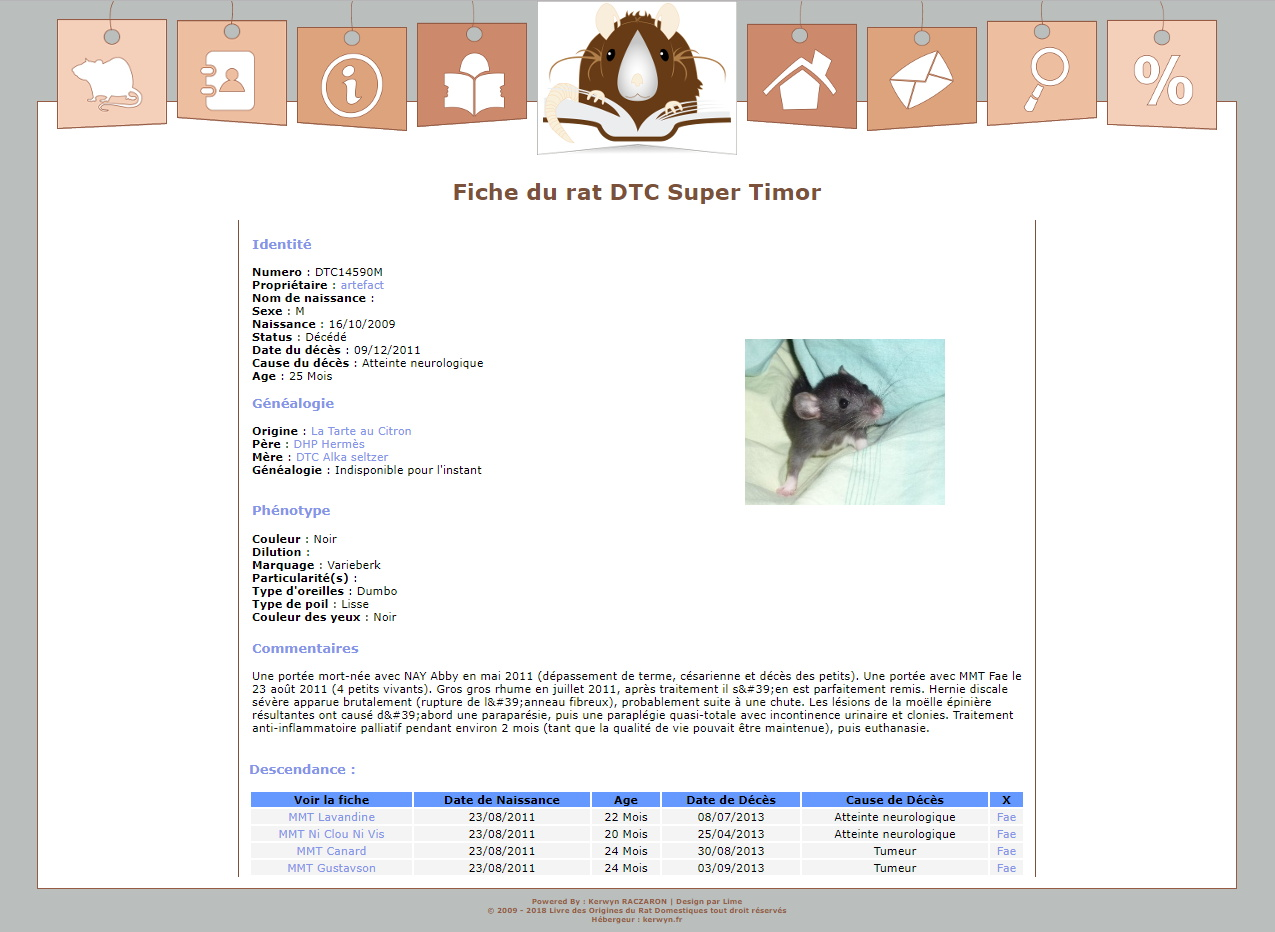
\includegraphics[width=0.8\linewidth]{FicheRat.jpg}\end{center}
\caption{Aperçu de la consultation d'une fiche rat (KerLORD).\label{fig:kerfiche}}
\end{figure}

\desire{Modifications V2.}
\begin{itemize}
\item Calculer et afficher l'âge en mois (âge actuel si vivant, âge au décès si mort) du rat dans la catégorie Identité (par exemple après « Statut » : Vivant ajouter « (xx mois) »).  
\item Liens pour consulter la fiche du propriétaire, la fiche de l'éleveur.
\end{itemize}

\subsection{Lister les fiches}
\existant{Fonctionnalités V1 à préserver.}
\begin{itemize}
\item Lister ses rats depuis son compte (onglets « Tous mes rats », « Mes femelles », « Mes mâles », « Mes rats décédés », « Mes fiches à corriger »). Maquette : figure~\ref{fig:kerdashuser}.   
\item Lister les enfants d'un rat (à insérer lors de la consultation de la fiche)  -- visible sur la maquette de la figure~\ref{fig:kerfiche}.
\end{itemize}

\begin{figure}[htbp!]
\begin{center}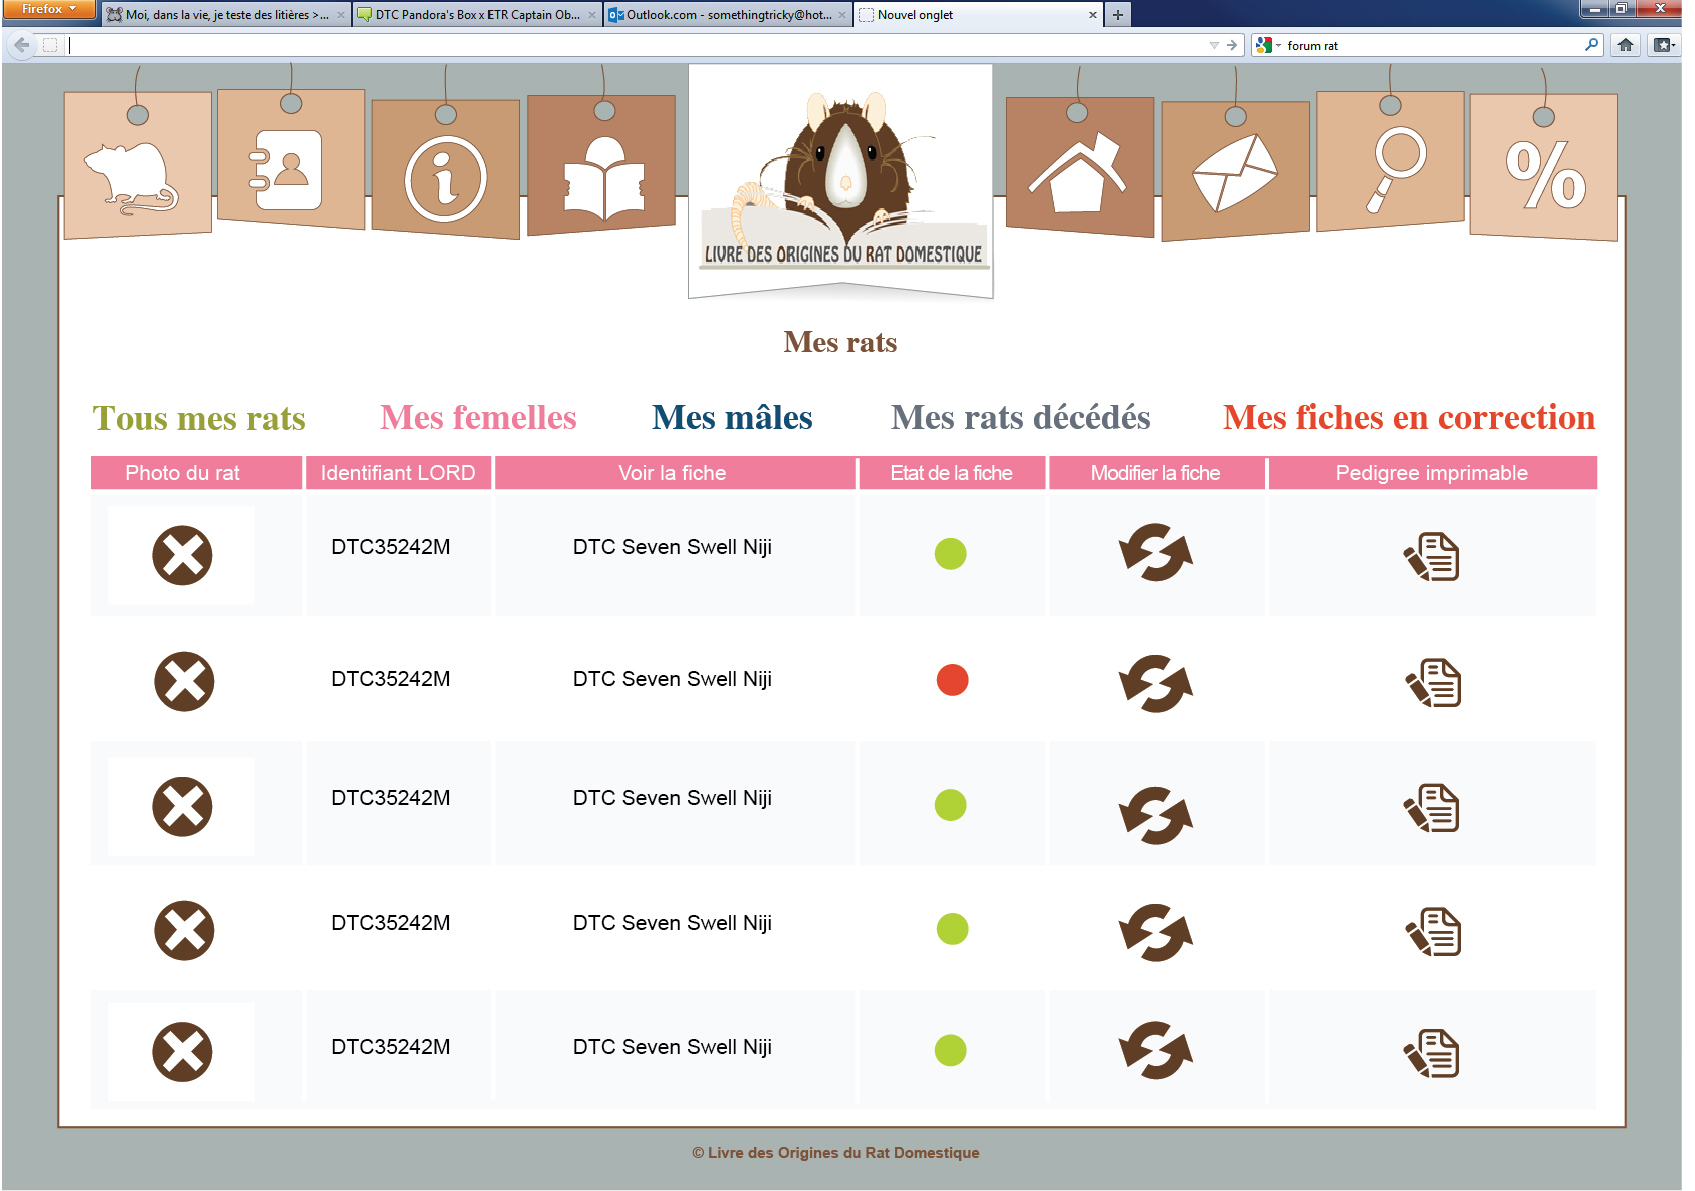
\includegraphics[width=0.8\linewidth]{DashboardUser.jpg}\end{center}
\caption{Aperçu du panneau de la liste des rats d'un utilisateur (KerLORD).\label{fig:kerdashuser}}
\end{figure}

\desire{Modifications V2.}
\begin{itemize}
\item Calculer et afficher l'âge en mois (âge actuel si vivant, âge au décès si mort) dans la liste des descendants.
\item Afficher les rats dont les fiches sont au SAV, avec une mention (fiche non validée) 
\item Lister tous les rats d'un propriétaire depuis sa fiche utilisateur
\item Lister tous les rats nés dans une raterie depuis sa fiche raterie
\item Lister tous les rats d'une portée depuis la fiche portée
\end{itemize}

\subsection{Générer la généalogie}
\existant{V1.} Un tableau hmtl est généré par la lecture récursive des parents, dans une limite de 5 générations. Chaque case reprend les informations principales de l'ascendant et peut être cliquée pour revenir à sa fiche individuelle. 
\desire{Ajout de fonctionnalités en V2 :} 
\begin{itemize}
\item Colorier les rats apparaissant plusieurs fois dans la généalogie (couleur unique par individu sur la généalogie affichée.)
\item Générer un pdf téléchargeable
\item Améliorer la visualisation (aspect ratio des cases, informations affichées, proposer une généalogie circulaire ?).
\end{itemize}

\subsection{Rechercher un ou des rats}

\existant{V1.} Maintien des possibilités actuelles de recherche, sauf champ « reproductible ».  
\desire{V2.} Ajout d'une recherche par fourchette de date de naissance (né avant le..., après le...).

\section{Fonctionnalités rateries}

\subsection{Enregistrer une raterie}

\desire{\`A ajouter en V2.} 
\begin{itemize}
\item Afficher un texte d'avertissement rappelant que l'enregistrement d'une raterie n'est possible que si l'utilisateur a déjà eu une portée née chez lui, ou une portée en collaboration.
\item Vérification que l'affixe et le nom sont disponibles. 
\item Prise en charge des caractères spéciaux (apostrophes, tirets)
\end{itemize}

\subsection{Modifier une raterie}
Réservé aux utilisateurs enregistrés.

\subsection{Afficher une raterie}
Afficher nom du propriétaire, site web, localisation (département ou code postal), présentation. Boutons pour lister les portées, lister les rats nés sous cet affixe.
\subsection{S'enregistrer dans l'annuaire}
Réservé aux utilisateurs enregistrés.

Signaler que le code postal est obligatoire si la raterie souhaite être affichée dans la carte des rateries.

\section{Fonctionnalités portées}

\subsection{Enregistrer une portée}
Réservé aux utilisateurs enregistrés.

\subsection{Modifier une de ses portées} 

\subsection{Afficher une portée} 

\subsection{Ajouter un raton à une de ses portées}
 
\desire{Ajout V2.} Lorsque les informations communes d'une portée ont été saisies (origine, date de naissance, ID des parents), possibilité de générer depuis la fiche portée un formulaire pré-rempli avec ces informations pour l'enregistrement d'un rat de la portée. (Bouton « ajouter un raton » ouvrant un nouvel onglet ?)  

\section{Fonctionnalités back office}
\label{sec:backoffice}
\existant{Fonctionnalités existant en V1 et problèmes.} Le back office offre essentiellement la liste de toutes les fiches en attente, les affichages sont (une ligne par fiche) : bouton suppression, ID du rat, nom du rat, propriétaire de la fiche, date de dernière modification de la fiche. Problème : pas de fonctions de tri, pas de différence visible entre fiche en attente d'action utilisateur et fiche en attente d'action modérateur, pas de notion de « modérateur en charge ».  

\subsection{Se connecter au back office}
\desire{Ajout V2.} 
\begin{itemize}
\item \sout{Réauthentification de l'utilisateur.} abandonné 
\item Affichage d'un « dashboard ».
\begin{itemize}
\item Infos synthétiques (nombre de fiches au SAV, dont nombre de fiches non traitées, nombre de fiches prises en charge par ce modérateur et qui attendent une action de sa part, date de la dernière action du modérateur...) Maquette indicative : figure~\ref{fig:kerdashback}. \desire{Liste précise et ordonnée à spécifier.}
\item Previews des fiches en attente par catégorie : fiches non traitées, fiches en attente de réponse utilisateur, fiches en attente de réponse SAV.
\end{itemize}
\item Accéder aux listes de chaque catégorie.
\item Fonctions de tri (toutes les fiches d'un même utilisateur, toutes les fiches attachées à une même portée...)
\end{itemize}

\begin{figure}[htbp]%
\begin{center}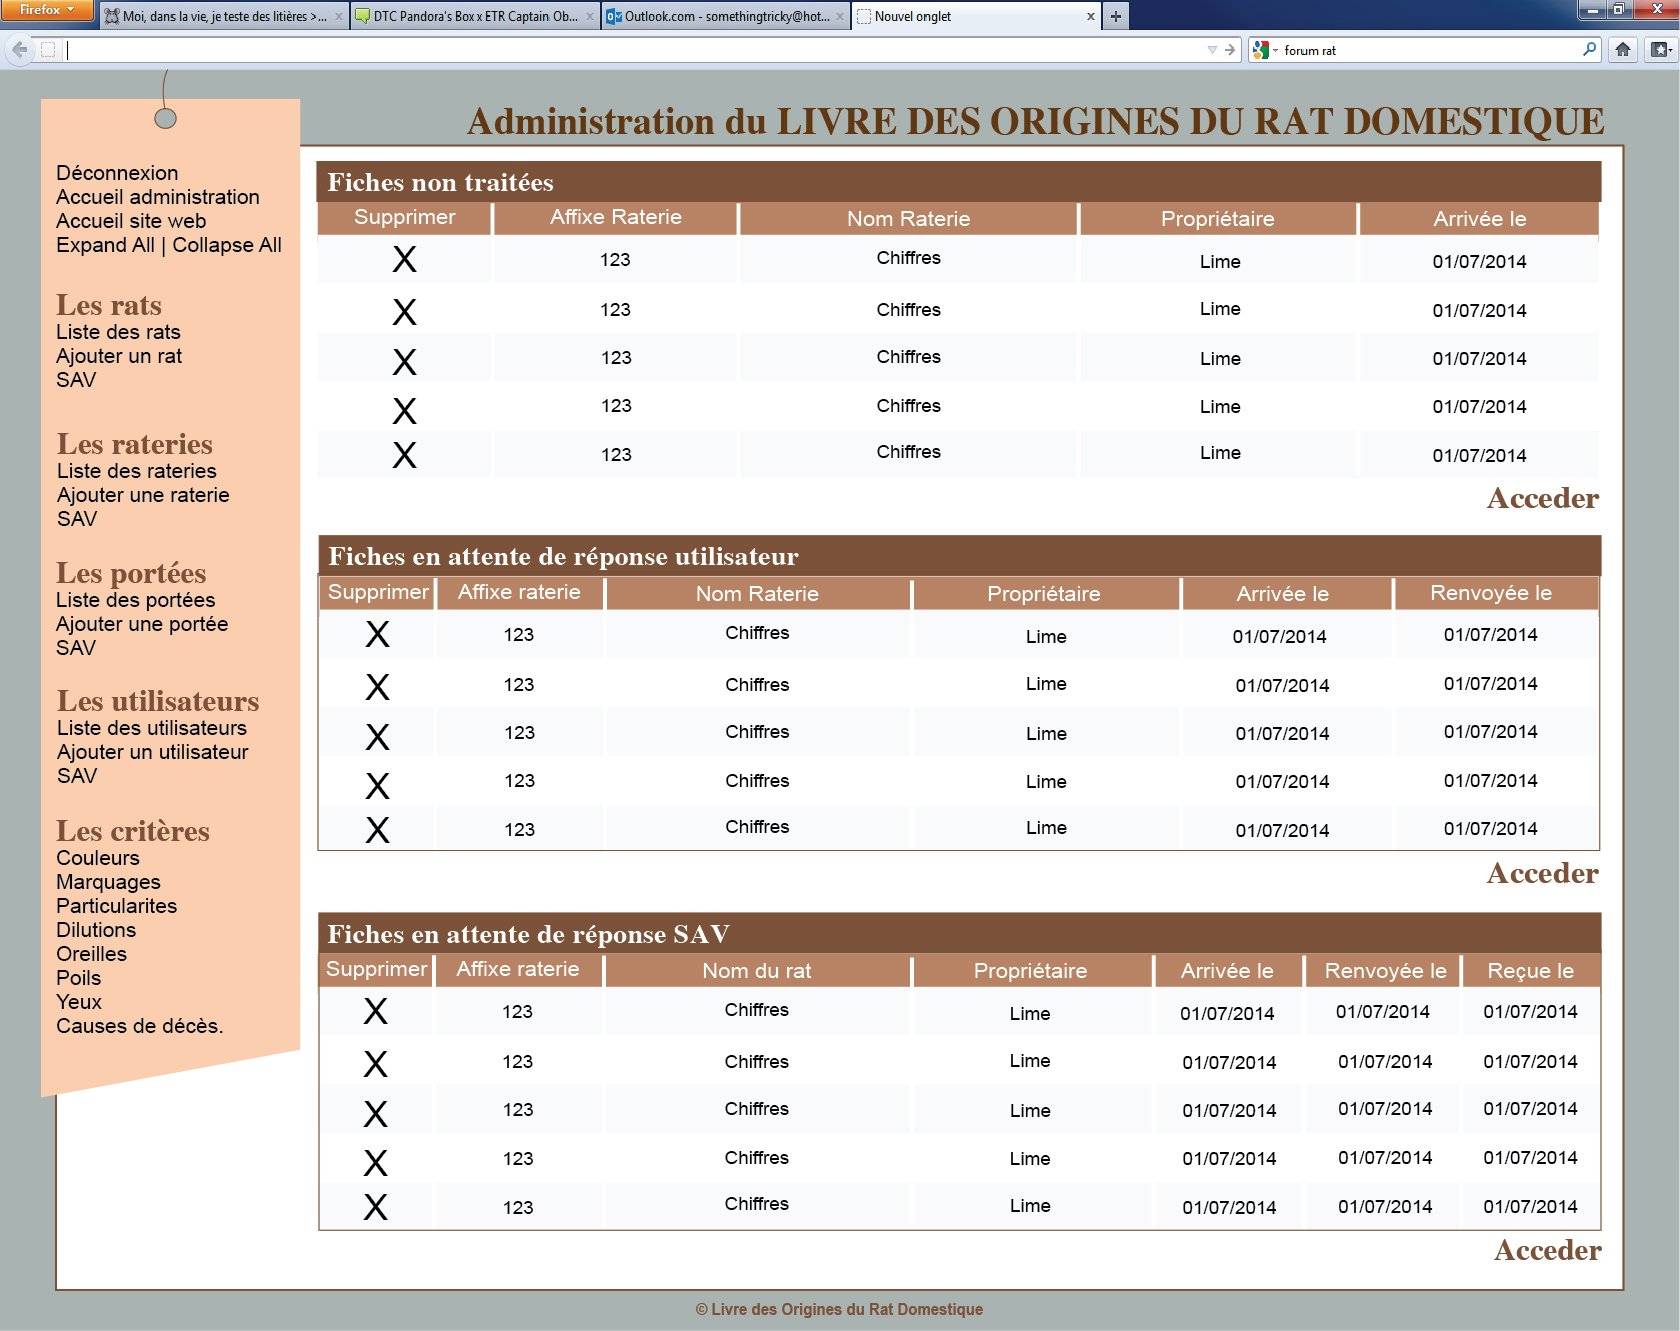
\includegraphics[width=0.8\linewidth]{MaquetteSAV.jpg}\end{center}
\caption{Maquette indicative du dashboard back-office.\label{fig:kerdashback}}
\end{figure}

\subsection{Lister les fiches jamais traitées (premier passage au SAV)}
Afficher la date d'arrivée de la fiche au SAV.

\subsection{Lister les fiches en attente de validation par un modérateur (après réponse de l'utilisateur)}
Afficher la date d'arrivée de la fiche au SAV, la date de la dernière réponse de l'utilisateur, le pseudo du modérateur qui traite la fiche.

\subsection{Lister les fiches en attente de modification par l'utilisateur}
Afficher la date d'arrivée de la fiche au SAV, la date de la dernière intervention d'un modérateur, le pseudo du modérateur qui traite la fiche.

\subsection{Intervenir sur une fiche rat}
\existant{Fonctions V1 à préserver.} Editer la fiche, la valider, laisser un commentaire à l'utilisateur (commentaire sur la fiche), la supprimer.

\desire{Ajouts V2.} Changer le statut d'une fiche (« en attente d'action d'un modérateur », « en attente de modification par l'utilisateur ».) Déclencher une communication avec l'utilisateur (envoi d'un mail et/ou d'un message privé.) Les actions déclenchent la mise à jour de la « date de dernière modification. »   

\subsection{Intervenir sur une fiche portée}
Idem.

\subsection{Intervenir sur une fiche raterie}
Idem.

\subsection{Intervenir sur un utilisateur}
\desire{V2.} Editer les informations de la fiche (pseudo, mail, etc.), déclencher une procédure de régénération de mot de passe. Ajout d'un commentaire consultable uniquement par les modérateurs. (Informations confidentielles, avertissements...)

\subsection{Communiquer avec un utilisateur}
Envoyer un message privé ou un mail à l'utilisateur depuis une de ses fiches en attente, depuis son profil.

\subsection{Déclencher des actions de masse}
\begin{itemize}
\item « Tuer » tous les rats âgés de plus de xx mois et encore vivants (positionner le champ \texttt{is\_alive} à 0 et les causes de décès à Cause inconnue / Aucune info)
\item « Désactiver » toutes les rateries n'ayant pas enregistré de portées depuis yy mois (positionner le champ \texttt{is\_alive} à 0, ne plus afficher dans la carte des rateries)
\end{itemize}


\section{Fonctionnalités secondaires}
\subsection{Messagerie interne}
Possibilité d'envoyer un message privé à un autre utilisateur depuis sa fiche. Consultation des messages reçus, suppression d'un message, etc. \desire{Sera limité aux conversations dont un des participants est un membre du staff (rôles root, admin, staff).}

\subsection{Calcul et affichage de statistiques}
Onglet statistiques du site, voir annexe~\ref{app:stats}.

\subsection{Responsiveness}
Version mobile du site ou application.

\subsection{Edition des pages « statiques » depuis le SAV}
Notices d'utilisation, mentions légales, message sur la page d'accueil...

\subsection{Courbe de poids}
\desire{Abandonné pour l'instant.} Pas prioritaire, garder la possibilité de le faire un jour.

\subsection{Internationalisation / gestion multilingue}
Trois langues prévues : anglais (langue du développement), français (dont les anglicismes en usage ; sera la langue par défaut pour la locale fr\_FR), « québécois » (traduction de tous les termes anglais en français).  

\subsection{Autres fonctionnalités mineures}
\begin{itemize}
\item 8.6.1 Redimensionnement auto des photos (avec imagemagick ?)
\item 8.6.2 Génération d'un PDF pour les généalogies
\item 8.6.3 Impression d'une fiche
\item 8.6.4 Conserver des brouillons de fiches avant envoi au SAV
\item 8.6.5 Calcul du taux de consanguinité d'un rat
\end{itemize}

\newpage
\appendix
\setlength{\parskip}{0pt}
\section{Annexes}

\subsection{Schémas des bases de données}

\subsubsection{Base V1 Production}
\label{app:dbv1}
Tables fonctionnelles :

\begin{center}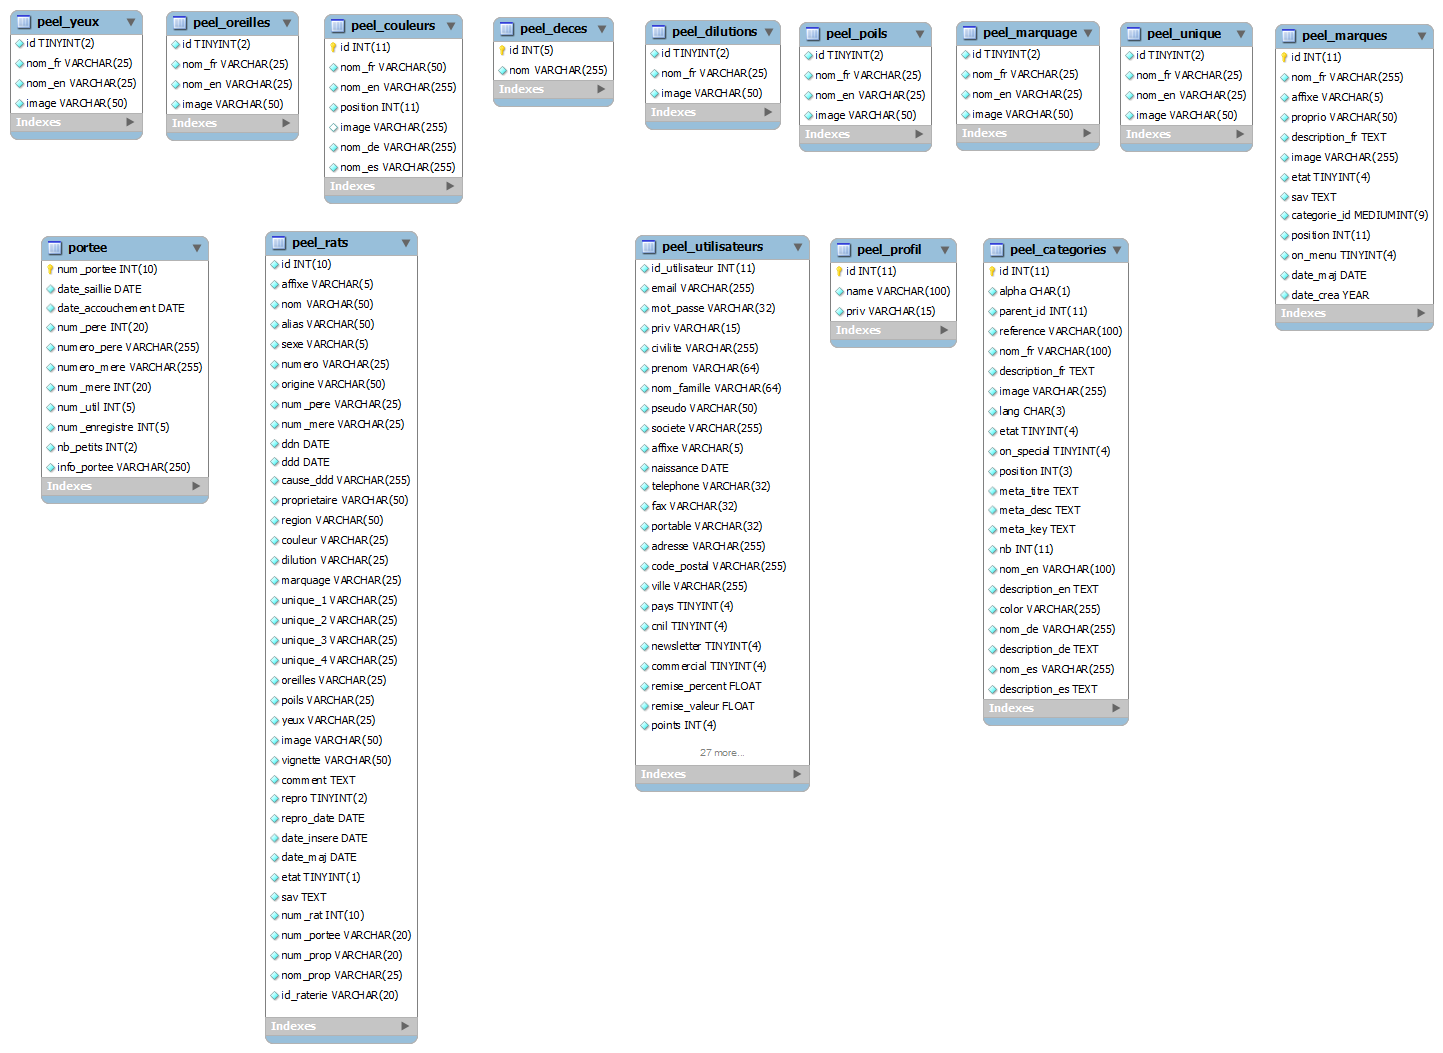
\includegraphics[width=\textwidth]{LORDv1_Tables_fonctionnelles.png}\end{center}

Tables techniques :

\begin{center}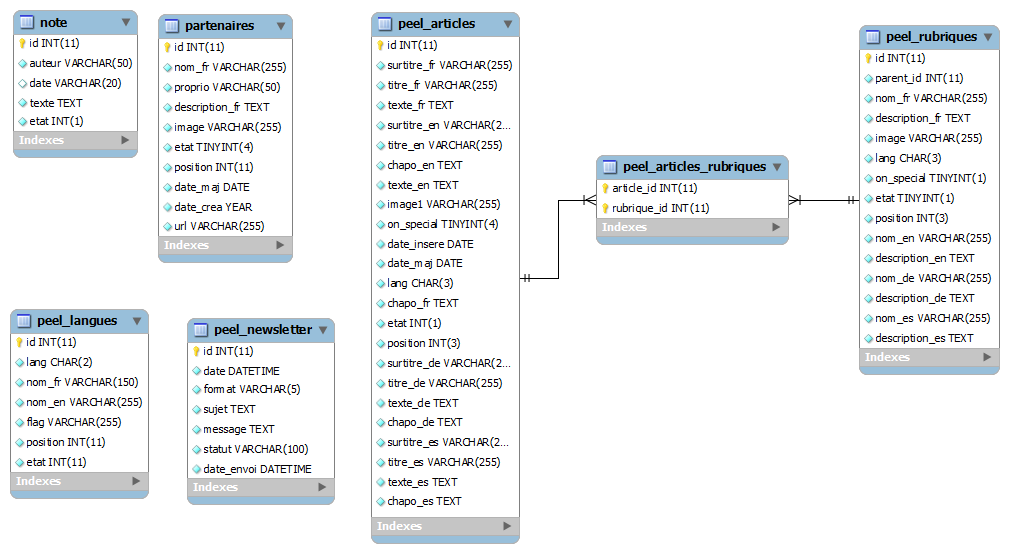
\includegraphics[width=0.75\textwidth]{LORDv1_Tables_techniques.png}\end{center}


\begin{landscape}
\subsubsection{Base V2 CakeLORD}
\label{app:dbv2}
\vspace*{\stretch{1}}
\noindent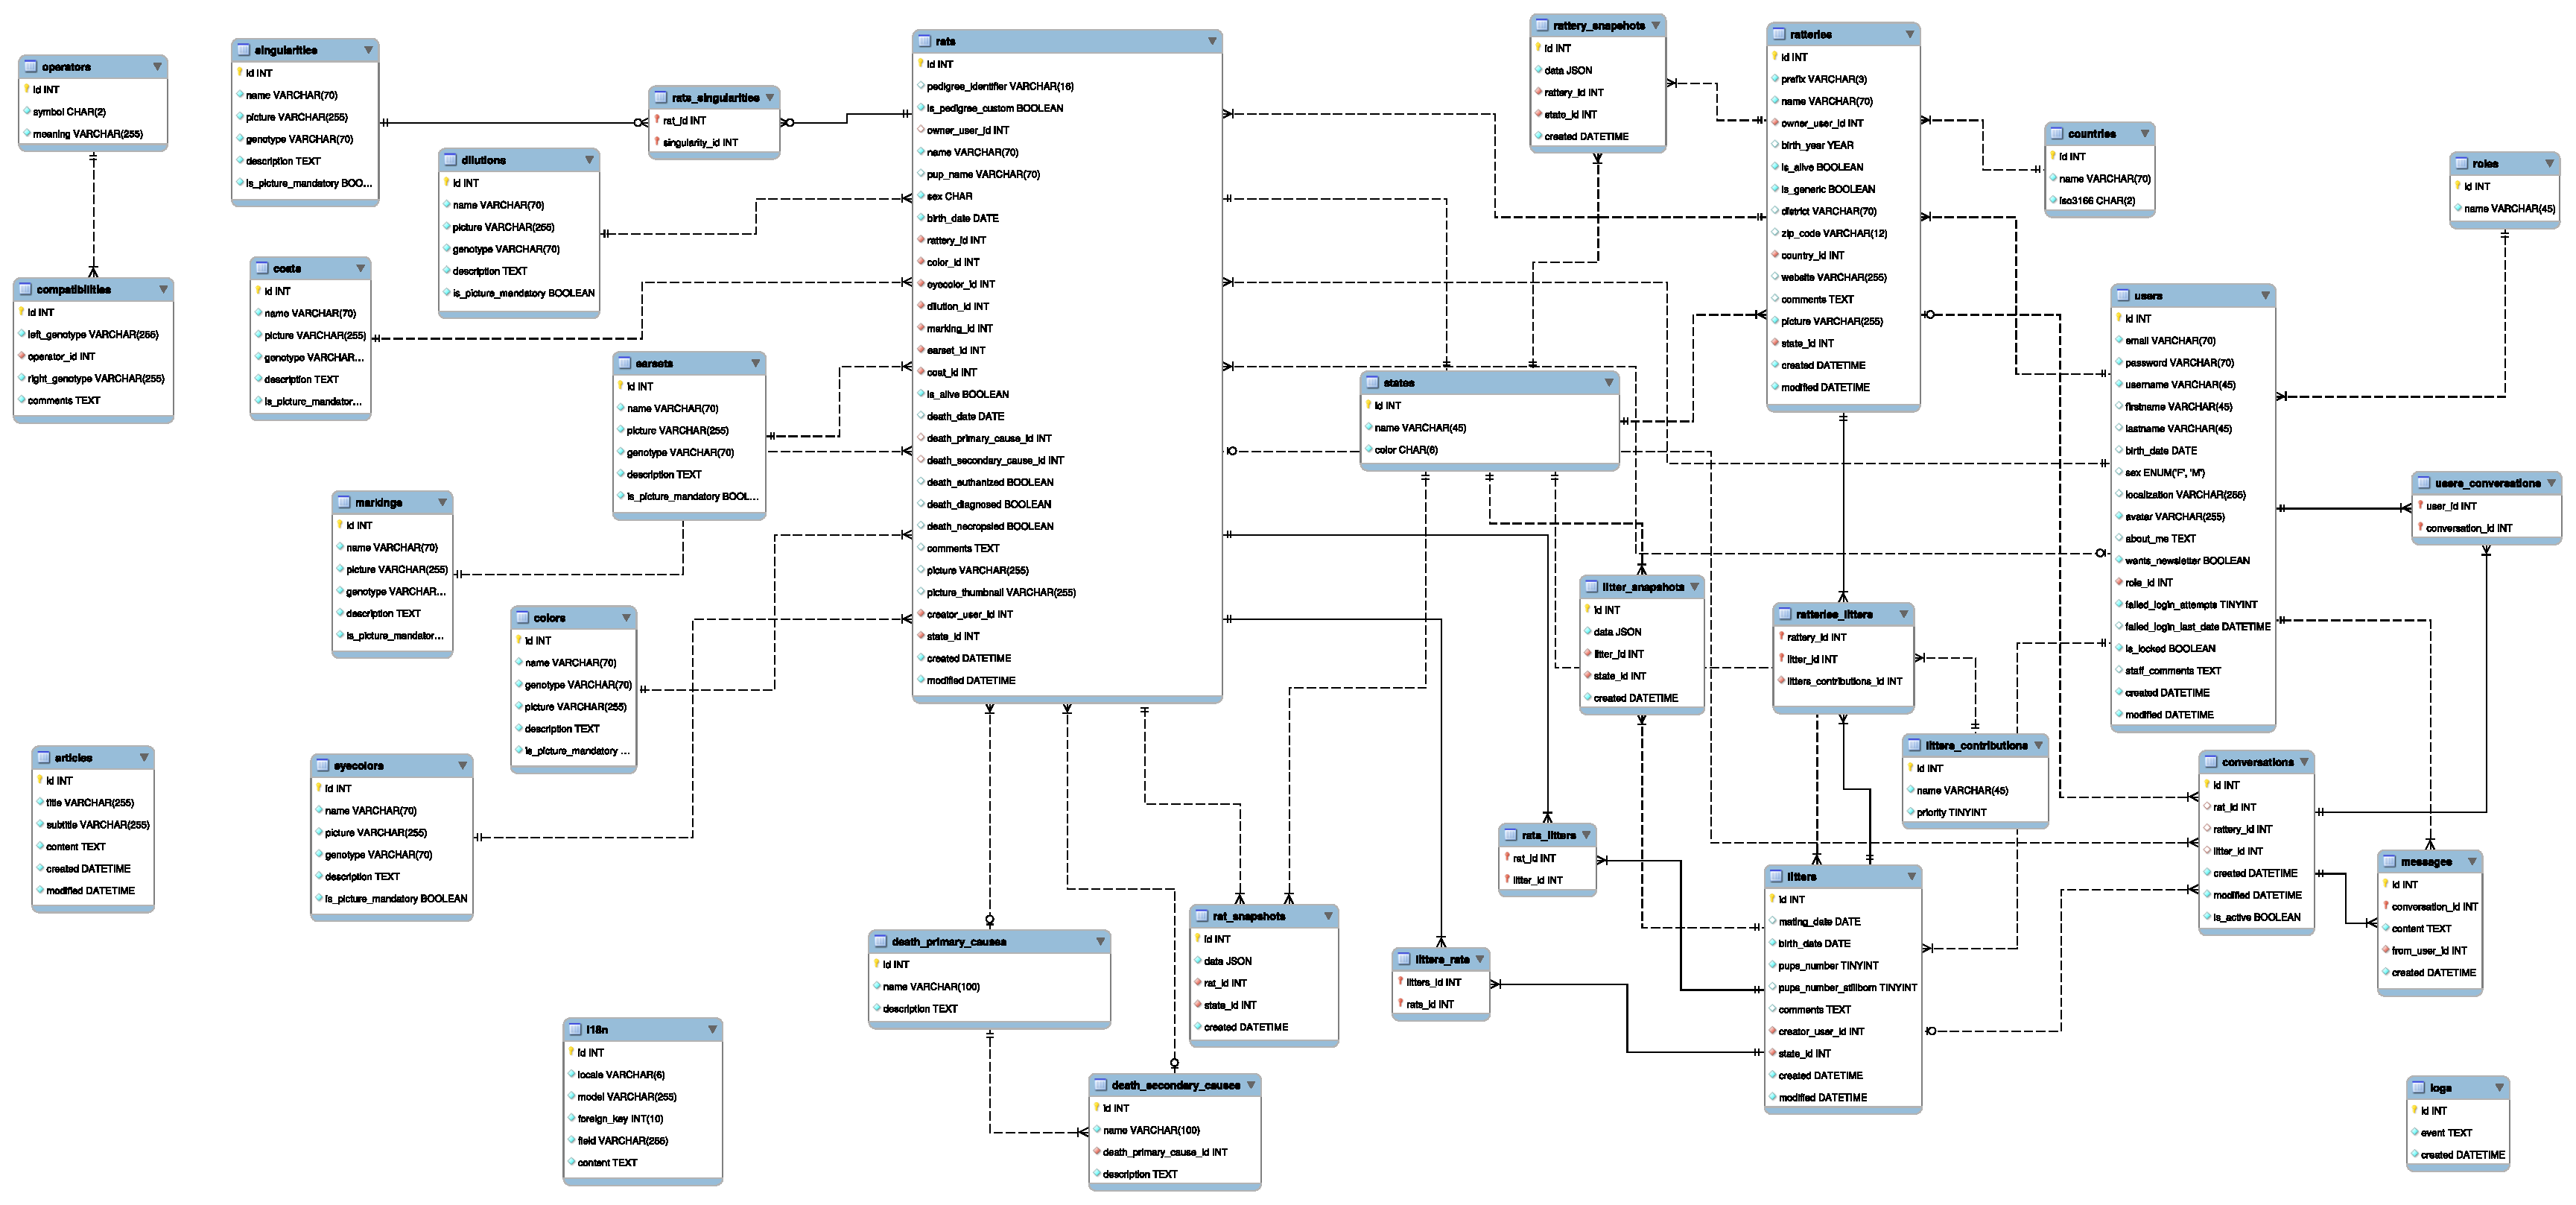
\includegraphics[width=\linewidth]{cakelord.eps}
\vspace*{\stretch{1}}
\end{landscape}

%\newpage
%\thispagestyle{empty}
%\begin{center}
%\rotatebox{90}{%
%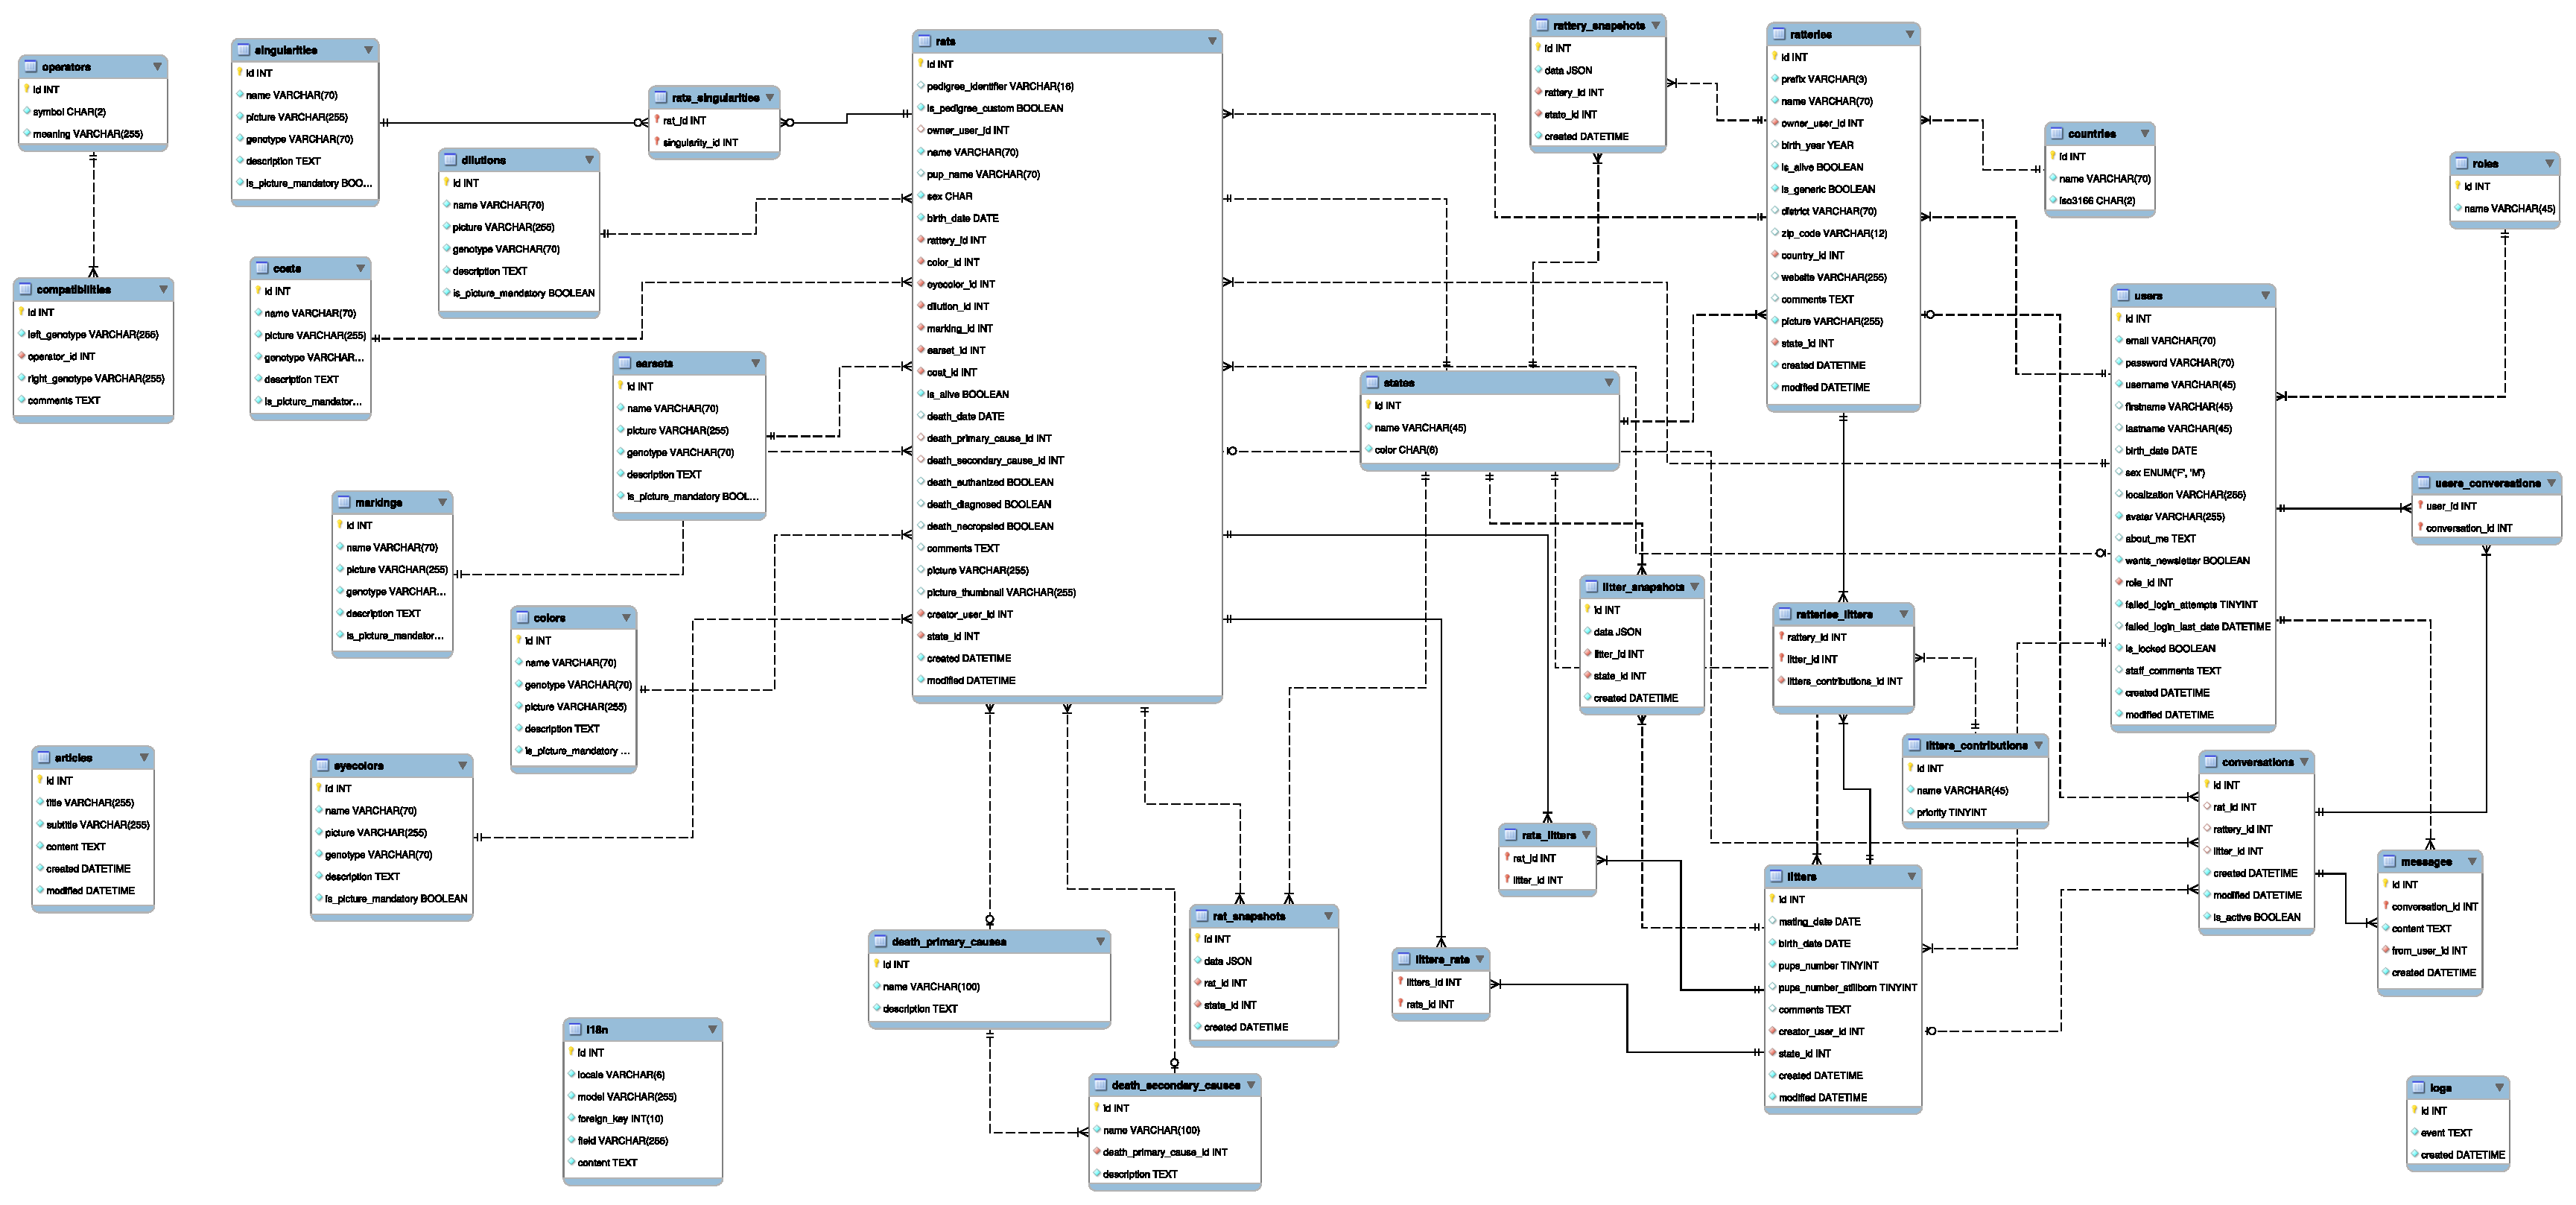
\includegraphics[width=\textheight]{cakelord.eps}
%}

\subsection{Liste des vérifications à l'enregistrement d'une fiche rat}
\label{app:verifs}
\small
%\noindent\begin{tabularx}{\textwidth}{|p{0.35cm}|p{1.35cm}|p{5cm}|X|}\hline
\noindent\begin{tabularx}{\textwidth}{|l|l|R|R|}\hline
\textbf{\#} & \textbf{Champ} & \textbf{Vérification} & \textbf{Message d'erreur}\\\hline

1 & Sexe & Vérifier qu'un sexe a été entré. & Veuillez choisir le sexe du rat, c'est obligatoire. \\\hline

2 & Nom & Vérifier qu'un nom a été entré. &Veuillez entrer un nom pour le rat, c'est obligatoire. \\\hline

3 & Nom & Vérifier que le nom n'est pas de la forme F+chiffre ou M+chiffre. & Les noms de type F1, M2... ne sont pas acceptés. Veuillez entrer un nom pour le rat ou attendre qu'il en ait un pour l'enregistrer. \\\hline

4 & Origine & Vérifier qu'au moins une fiche parent a été entrée, sauf si l'origine est une raterie générique & L'enregistrement d'un rat avec cet affixe n'est possible que si au moins un de ses parents possède une fiche. Merci de vérifier que vous avez choisi le bon affixe, et si oui, saisir le numéro d'identification du père ou de la mère. \\\hline

5 & ID père & Vérifier qu'il existe & Le numéro entré pour le père ne correspond pas à une fiche existante. Merci de vérifier votre saisie ou de créer la fiche du père si elle n'existe pas. \\\hline


6 & ID père & Vérifier qu'il s'agit d'un mâle & Le numéro entré pour le père correspond à une femelle. Merci de vérifier votre saisie.\\\hline


7 & ID mère & Vérifier qu'il existe & Le numéro entré pour la mère ne correspond pas à une fiche existante. Merci de vérifier votre saisie ou de créer la fiche de la mère si elle n'existe pas.\\\hline


8 & ID mère & Vérifier qu'il s'agit d'une femelle & Le numéro entré pour la mère correspond à un mâle. Merci de vérifier votre saisie. \\\hline


9 & DDN & Vérifier le format & La date de naissance doit être saisie au format JJ/MM/AAAA.\\\hline


10 & DDN & Vérifier que l'année n'est pas antérieure à 1900. & Pour des raisons de fiabilité des données, nous n'acceptons pas l'enregistrement de rats nés avant 1900. Merci de vérifier votre saisie.\\\hline


11 & DDN & Vérifier que la date de naissance n'est pas postérieure à la date du jour.& La date de naissance est impossible : ce jour n'a pas encore eu lieu.\\\hline


12 & DDN & S'il y a des fiches parents, vérifier que la date de naissance est postérieure à celle des parents & La date de naissance est impossible : rat né avant l'un de ses parents. Merci de vérifier votre saisie.\\\hline


13 & DDN & S'il y a une fiche pour la mère, vérifier que la date de naissance n'est pas postérieure à la date de décès de la mère. & La date de naissance est impossible : rat né après la mort de sa mère. Merci de vérifier votre saisie.\\\hline


14 & DDN & S'il y a une fiche pour le père, vérifier que la date de naissance n'est pas postérieure à la date de décès du père MOINS 24 jours. & La date de naissance est impossible : rat conçu après la mort de son père. Merci de vérifier votre saisie.\\\hline


15 & DDD & Vérifier le format & La date de décès doit être saisie au format JJ/MM/AAAA.\\\hline


16 & DDD & Vérifier qu'elle est postérieure à la date de naissance. & La date de décès est impossible : rat mort avant d'être né. Merci de vérifier votre saisie.\\\hline


17 & DDD & Vérifier qu'elle est antérieure à la date du jour. & La date de décès est impossible : ce jour n'a pas encore eu lieu. Merci de vérifier votre saisie.\\\hline


18 & CDD & Si la cause est « vieillesse », vérifier que l'âge de décès est supérieur à 2 ans. & Vous avez indiqué que votre rat est mort de vieillesse, mais il n'avait que xxx mois. Merci de vérifier la date et la cause de décès.\\\hline


19 & CDD & Si la cause est dans la catégorie mortalité infantile, vérifier que l'âge de décès est inférieur à 6 semaines. & Vous avez indiqué que votre rat est mort d'une cause infantile, mais il avait plus de 6 semaines. Merci de vérifier la date et la cause de décès.\\\hline


20 & CDD & Si la cause est un des items « Autre problème... », vérifier la présence d'un commentaire. & Pour toute cause de décès de type « Autre problème », merci de préciser la cause exacte en commentaires. Si vous l'ignorez, ne choisissez pas de niveau 2 de cause de décès.\\\hline

\end{tabularx}
\normalsize

\subsubsection{Vérifications supplémentaires}

Si le temps le permet : 

\begin{itemize}
\item Etablir une liste de couleurs pour lesquelles la photographie est obligatoire. Si cette couleur est sélectionnée et qu'il n'y a pas eu de photos, envoyer le message d'erreur : (Vous avez choisi une couleur rare pour ce rat. Pour des raisons de fiabilité des données, merci d'ajouter une photographie permettant de bien apprécier sa couleur.) \desire{Mis en place par un champ \texttt{is\_picture\_mandatory} dans les tables techniques de traits physiques, liste à spécifier.}
\item Etablir une liste de combos impossibles, par exemple "siamois beige" ou "bleu perle". (Vous avez choisi un phénotype impossible. Merci de corriger votre saisie. En cas de doute sur le phénotype du rat, merci de contacter l'équipe à l'adresse ... - compléter ici avec l'endroit où se trouvera le forum SAV.) \desire{Mis en place par la table technique \texttt{compatibilities}, liste à spécifier.}
\item \sout{Etablir deux listes des couleurs, base noire et base agoutie, et vérifier que les deux parents ne sont pas de base noire si la couleur entrée est de base agoutie. (Vous avez choisi un phénotype impossible : deux parents de base noire ne peuvent engendrer des enfants de base agoutie. Merci de corriger votre saisie. En cas de doute sur le phénotype du rat, merci de contacter l'équipe à l'adresse ... - compléter ici avec l'endroit où se trouvera le forum SAV.)} \desire{Sera difficile sans modélisation complète de la génétique, abandonné pour l'instant.}
\end{itemize}

Champs nom / date de naissance / oreilles / yeux/ poils obligatoires pour valider une fiche. Couleur et Marquage obligatoires sauf exceptions à gérer comme certaines dilutions (par exemple, si albinos, marquage inconnu autorisé.) \desire{Mis en place par la table technique \texttt{compatibilities}, liste à spécifier.}

\subsection{Nouvelle liste des couleurs et correspondance}
\subsubsection{Nouvelle liste}

Agouti

Ambre (Agouti + PED)
 
Ambre bleu   (Agouti + PED + Bus)
 
Ambre dove   (Agouti + PED + Mink + Br)
 
Ambre dove mock   (Agouti + PED + Mock + Br)
 
Ambre lavande (Agouti + PED + Mink +   Bus)
 
Ambre lavande mock (Agouti + PED + Mock   + Bus)
 
Ambre mink   (Agouti + PED + Mink)
 
Ambre mock (Agouti + PED + Mock)
 
Ambre russe (Agouti + PED + Br)
 
Beige (Noir + RED)
 
Beige dove (Noir   + RED + Mink + Br )
 
Beige dove mock (Noir + RED + Mock + Br)
 
Beige mink (Noir   + RED + Mink)
 
Beige mock (Noir + RED + Mock)
 
Beige russe (Noir + RED + Br)
 
Bleu russe
 
Bleu russe agouti (Agouti + Br)
 
Bleu us
 
Bleu us agouti   (Agouti + Bus)
 
Cannelle (Agouti + Mink)
 
Cannelle mock (Agouti + Mock)
 
Champagne (Noir + PED)
 
Champagne mink (Noir + PED + Mink)

Champagne mock(Noir + PED + Mock)
 
Champagne russe (Noir + PED + Br)
 
Chocolat
 
Double bleu (Noir + Bus + Br)
 
Double bleu agouti (Agouti + Bus + Br)
 
Double canelle bleu (Agouti + Mink +   Mock + Bus)
 
Double canelle russe (Agouti + Mink + Mock + Br)
 
Double cannelle (Agouti + Mink + Mock)
 
Double havane ( Noir + Mink + Mock +   porteur RED)
 
Double havane agouti ( Agouti + Mink +   Mock + porteur RED)
 
Double havane russe (Noir + Mink + Mock   + Br + porteur RED)
 
Double havane russe agouti (Agouti +   Mink + Mock + Br + porteur RED)
 
Double lilas (Noir + Mink + Mock + Bus +   porteur RED)
 
Double lilas agouti (Agouti + Mink +   Mock + Bus + porteur RED)
 
Double mink (Noir + Mink + Mock)
 
Double mink bleu (Noir + Mink + Mock +   Bus)
 
Double mink russe (Noir + Mink + Mock +   Br)
 
Double moka (Noir + Mink + Mock +   porteur PED)
 
Double moka agouti (Agouti + Mink + Mock   + porteur PED)
 
Double moka bleu (Noir + Mink + Mock +   Bus + porteur PED)
 
Double moka bleu agouti (Agouti + Mink +   Mock + Bus + porteur PED)
 
Double moka russe (Noir + Mink + Mock +   Br + porteur PED)
 
Double moka russe agouti (Agouti + Mink   + Mock + Br + porteur PED)
 
Dove (Noir + Mink + Br)
 
Dove agouti   (Agouti + Mink + Br)
 
Dove mock (Noir + Mock + Br)
 
Dove mock agouti   (Agouti + Mock + Br)
 
Graphite
 
Havane (Noir + Mink + porteur RED)
 
Havane agouti (Agouti + Mink + porteur   RED)
 
Havane mock (Noir + Mock + porteur RED)
 
Havane mock agouti (Agouti + Mock +   porteur RED)
 
Havane russe (Noir + Mink + Br + porteur   RED)
 
Havane russe agouti (Agouti + Mink + Br   + porteur RED)

Havane russe mock (Noir + Mock + Br + porteur RED)
 
Havane russe mock agouti (Agouti + Mock + Br + porteur RED)

Ice (Noir + PED + Bus)
 
Ice mink (Noir + PED + Mink + Bus)
 
Ice mock (Noir + PED + Mock + Bus)
 
Lavande (Noir + Mink + Bus)
 
Lavande agouti(Agouti + Mink + Bus)
 
Lavande mock (Noir + Mock + Bus)
 
Lavande mock agouti (Agouti + Mock + Bus)
 
Lilas (Noir + Mink + Bus + porteur RED)
 
Lilas agouti (Agouti + Mink + Bus +   porteur RED)
 
Lilas mock (Noir + Mock + Bus + porteur RED)

Lilas mock agouti (Agouti + Mock + Bus + porteur RED)
 
Mink
 
Mock
 
Moka (Noir + Mink + porteur PED)
 
Moka agouti (Agouti + Mink + porteur   PED)
 
Moka bleu (Noir + Mink + Bus + porteur   PED)
 
Moka bleu agouti (Agouti + Mink + Bus +   porteur PED)
 
Moka bleu mock (Noir + Mock + Bus + porteur PED)
 
Moka bleu mock agouti (Agouti + Mock +   Bus + porteur PED)
 
Moka mock (Noir + Mock + porteur PED)
 
Moka mock agouti (Agouti + Mock +   porteur PED)
 
Moka russe (Noir + Mink + Br + porteur  PED)
 
Moka russe agouti (Agouti + Mink + Br +  porteur PED)
 
Moka russe mock (Noir + Mock + Br + porteur PED)
 
Moka russe mock agouti (Agouti + Mock +  Br + porteur PED)
 
Noir
 
Platine (Noir + RED + Bus)
 
Platine mink (Noir + RED + Mink + Bus)
 
Platine mock (Noir + RED + Mock + Bus)
 
Topaze (Agouti + RED)
 
Topaze bleu (Agouti + RED + Bus)
 
Topaze dove (Agouti + RED + Mink + Br)
 
Topaze dove mock (Agouti + RED + Mock + Br)
 
Topaze mink (Agouti + Mink + RED)
 
Topaze mock (Agouti + RED + Mock)
 
Topaze russe (Agouti + RED + Br)

\desire{Warning ergonomie.} Cette liste est très longue, l'ergonomie pour l'entrée d'un rat par menu déroulant sera mauvaise. Il faudrait envisager une saisie en plusieurs étapes comme pour les causes de décès, par exemple : choisir d'abord si base agoutie ou noire, puis une famille de couleurs (« tous les ambres », « tous les topazes »...), puis les variantes attachées (« ambre », « ambre bleu », « ambre dove »...)         

\subsubsection{Correspondance}

\begin{center}\begin{tabular}{|l|l|}\hline
\textbf{Ancienne couleur} & \textbf{Nouvelle couleur} \\\hline
Agouti& Agouti  \\\hline
Agouti dove mock& Dove mock agouti (Agouti + Mock + Br) \\\hline
Ambre& Ambre (Agouti + PED)\\\hline
Ambre base vison& Ambre mink   (Agouti + PED + Mink)\\\hline
Argent& à supprimer \\\hline
Beige& Beige (Noir + RED)\\\hline
Beige base mink& Beige mink  (Noir   + RED + Mink)\\\hline
Beige base mock& Beige mock  (Noir   + RED + Mock)\\\hline
Bleu polaire russe& Champagne russe (Noir + PED + Br)\\\hline
Bleu russe& Bleu russe (Noir + Br)\\\hline
Bleu russe agouti& Bleu russe agouti (Agouti + Br)\\\hline
Bleu us& Bleu us (Noir + Bus)\\\hline
Bleu us agouti& Bleu us agouti (Agouti + Bus)\\\hline
Cannelle& Cannelle (Agouti + Mink)\\\hline
Cannelle mock& Cannelle mock (Agouti + Mock)\\\hline
Champagne& Champagne (Noir + PED)\\\hline
Champagne base mink& Champagne mink (Noir + PED + Mink)\\\hline
Chocolat& Chocolat \\\hline
Double bleu& Double bleu (Noir + Bus + Br)\\\hline
Double bleu agouti& Double bleu agouti (Agouti + Bus + Br)\\\hline
Double cannelle& Double cannelle (Agouti + Mink + Mock)\\\hline
Double cannelle beige & à supprimer \\\hline
Double mink& Double mink (Noir + Mink + Mock)\\\hline
Dove& Dove (Noir + Mink + Br)\\\hline
Dove agouti& Dove Agouti (Agouti + Mink + Br)\\\hline
Dove mock& Dove mock (Noir + Mock + Br)\\\hline
Graphite& Graphite\\\hline
Havane& Havane (Noir + Mink + porteur RED)\\\hline
Havane agouti& Havane agouti (Agouti + Mink + porteur RED)\\\hline
Ice&  Ice (Noir + PED + Bus)\\\hline
Lavande& Lavande (Noir + Mink + Bus)\\\hline
Lavande agouti& Lavande agouti (Agouti + Mink + Bus)\\\hline
Lavande mock& Lavande mock (Noir + Mock + Bus)\\\hline
Mink& Mink \\\hline
Mock& Mock \\\hline
Mock Havane& Havane mock (Noir + Mock + porteur RED)\\\hline
Mock Havane Agouti& Havane mock agouti (Agouti + Mock + porteur RED)\\\hline
Mock mink& Mock (Noir + Mock)\\\hline
Noir& \\\hline
Platine agouti& Topaze bleu (Agouti + RED + Bus)\\\hline
Platine base PED& Champagne bleu (Noir + PED + Bus)\\\hline
Platine base RED& Platine (Noir + RED + Bus)\\\hline
Platine base beige& Platine (Noir + RED + Bus)\\\hline
Platine base mink& Platine mink (Noir + RED + Mink + Bus)\\\hline
Platine mock& Platine mock (Noir + RED + Mock + Bus)\\\hline
Platine russe& Beige russe (Noir + RED + Br)\\\hline
Platine russe agouti& Topaze russe (Agouti + RED + Br)\\\hline
Silver Fawn& Topaze mink (Agouti + Mink + RED)\\\hline
Topaze& Topaze (Agouti + RED)\\\hline
Topaze base mink& Topaze mink (Agouti + Mink + RED)\\\hline
Topaze mock& Topaze mock (Agouti + Mock + RED)\\\hline
\end{tabular}\end{center}

\subsection{Autres listes de traits physiques}

Dilutions : 
\begin{itemize}
\item Albinos
\item \sout{BED - Black Eyed Devil}
\item \sout{BEH - Black Eyed Himalayan}
\item \sout{BES - Black Eyed Siamese}
\item Burmese himalayen
\item Burmese sable himalayen
\item Burmese sable siamois
\item Burmese siamois
\item Biscuit (burmese albinos)
\item \desire{Ajout : Devil}
\item Himalayen
\item \sout{Ivory (albinos yeux noirs)}
\item \sout{RED - Red Eyed Devil}
\item Siamois
\item Aucune
\end{itemize}

\desire{NB.} Suppression de toutes les dilutions contenant une notion de couleur d’yeux, qui sera exclusivement gérée par le champ couleur des yeux. Ajout de la dilution Biscuit.

Marquages : suppression de tous les marquages contenant une notion de couleur d’yeux (BEW/PEW/REW), seront fusionnés dans un marquage « Blanc surmarqué ». 

Particularités : suppression de la particularité Black-Eyed (sera gérée par la couleur des yeux.) \desire{Liste à spécifier avec ses incompatibilités.}

\subsection{Nouvelle liste des décès et correspondance}
\subsubsection{Liste des catégories de décès (cause de décès niveau 1)}

\begin{enumerate}
\item Cause inconnue
\item Accidents, traumatismes, intoxications
\item Cardio-vasculaire
\item Digestif
\item Mortalité infantile (moins de 6 semaines)
\item Muscles et squelette
\item Neurologique (cerveau, moelle épinière, nerfs)
\item Œil, oreille, bouche, face
\item Peau
\item Respiratoire
\item Système reproducteur
\item Système urinaire (reins, vessie)
\item Vieillesse, mort naturelle (24 mois minimum)
\item Autres
\end{enumerate}

\subsubsection{Liste des causes de décès (cause de décès niveau 2)}

\begin{enumerate}
\item Cause inconnue
\begin{enumerate}
\item Aucune information (présumé mort)
\item Cause indéterminée (date connue)
\end{enumerate}
\item Accidents, traumatismes, intoxications
\begin{enumerate}
\item Accident domestique (écrasement, accident de porte…)
\item Accident vétérinaire (anesthésie lors d’une opération mineure, erreur médicale…)
\item Bagarres, blessures, morsures graves, hémorragie consécutive (hors hémorragie anormale)
\item Brûlures thermiques ou chimiques
\item Chutes, fractures, traumatisme crânien ou de la moelle épinière (hors bagarres)
\item Coup de chaleur
\item Étouffement, fausse route
\item Empoisonnement (produits ménagers, poisons, médicaments volés…)
\item Intoxication alimentaire
\item Surdosage médicamenteux (médicaments vétérinaires prescrits)
\item Autre accident ou traumatisme
\end{enumerate}
\item Cardio-vasculaire
\begin{enumerate}
\item Crise cardiaque, infarctus, embolie pulmonaire
\item Insuffisance cardiaque, valvulopathie
\item Hémorragie (exagérée par rapport au contexte, anomalie de la coagulation, hémophilie)
\item Autre problème cardiaque ou vasculaire
\end{enumerate}
\item Digestif
\begin{enumerate}
\item Abcès digestif
\item Gastro-entérite, diarrhée
\item Hémorragie digestive
\item Insuffisance hépatique
\item Malnutrition
\item Mégacôlon héréditaire
\item Occlusion intestinale (hors mégacôlon)
\item Prolapsus rectal
\item Tumeur digestive (estomac, foie, pancréas, intestins…)
\item Autre problème digestif
\end{enumerate}
\item Mortalité infantile (moins de 6 semaines)
\begin{enumerate}
\item Malformation, hydrocéphalie
\item Manque de lait
\item Mort-né
\item Autre cause de mort infantile
\end{enumerate}
\item Muscles et squelette
\begin{enumerate}
\item Infection / abcès musculaire
\item Infection articulaire ou osseuse, arthrite septique
\item Tumeur musculaire
\item Tumeur osseuse
\item Autre problème du système locomoteur
\end{enumerate}
\item Neurologique (cerveau, moelle épinière, nerfs)
\begin{enumerate}
\item Accident vasculaire cérébral
\item Atteinte progressive de la moelle épinière, paralysie dégénérative
\item Epilepsie
\item Infection du cerveau, encéphalite, méningite
\item Tumeur cérébrale
\item Tumeur hypophysaire (pituitaire)
\item Autre problème neurologique
\end{enumerate} 
\item Œil, oreille, bouche, face
\begin{enumerate}
\item Abcès dentaire
\item Abcès facial (hors dentaire et Zymbal)
\item Abcès rétro-orbitaire
\item Glaucome
\item Malocclusion dentaire
\item Otite, abcès dans l'oreille
\item Tumeur de la glande de Zymbal
\item Tumeur de la face (hors Zymbal)
\item Tumeur rétro-orbitaire
\item Autre problème touchant la tête
\end{enumerate}
\item Peau
\begin{enumerate}
\item Abcès sous-cutané
\item Infection étendue de la peau (pyodermite, escarres…)
\item Pododermatite
\item Tumeur cutanée, cancer de la peau
\item Autre problème de peau
\end{enumerate}
\item Respiratoire
\begin{enumerate}
\item Bronchite, pneumonie
\item Œdème pulmonaire
\item Tumeur pulmonaire, métastases pulmonaires
\item Autre problème respiratoire
\end{enumerate}
\item Système reproducteur
\begin{enumerate}
\item Complications de gestation ou de mise-bas
\item Infection de l'utérus (métrite, pyomètre)
\item Prolapsus vaginal (hors tumeurs et postpartum)
\item Tumeur mammaire
\item Tumeur ovarienne
\item Tumeur utérine
\item Tumeur vaginale
\item Tumeur de la prostate
\item Tumeur testiculaire
\item Tumeur des glandes préputiales
\item Autre problème du système reproducteur
\end{enumerate}
\item Système urinaire (reins, vessie)
\begin{enumerate}
\item Infection urinaire ou rénale
\item Insuffisance rénale
\item Obstruction de l’urètre, rétention urinaire, calculs
\item Tumeur de la vessie
\item Tumeur du rein
\item Autre problème du système urinaire
\end{enumerate}
\item Vieillesse, mort naturelle (24 mois minimum)
\item Autres
\begin{enumerate}
\item Allergie, choc anaphylactique
\item Cancer généralisé, leucémie, lymphome
\item Diabète
\item Euthanasie sans cause médicale
\item Infection / abcès indéterminé
\item Parasites
\item Septicémie
\item Tumeur autre (salivaire, splénique, surrénale, thyroïde...)
\item Tumeur indéterminée (organe atteint inconnu)
\item Virus, épidémie, déficience immunitaire (SDA, Sendaï, Tyzzer...)
\item Autre cause connue ne rentrant dans aucune catégorie
\end{enumerate}
\end{enumerate}

\desire{NB.} Sur la liste de correspondances suivante, l'astérisque désigne les fiches qui devront être repassées en « à valider par un modérateur » lors de la migration, pour vérification de la cause réelle de décès si possible. (En principe, nombre relativement réduit de fiches.)  

\subsubsection{Correspondance anciennes causes vers nouvelles causes}
\small

\noindent\begin{tabularx}{\textwidth}{|l|R|R|}\hline
\textbf{Ancienne cause} & \textbf{Nouvelle cause niveau 1} & \textbf{Nouvelle cause niveau 2}\\\hline
Accident domestique & 2. Accidents, traumatismes & 2.1 Accident domestique \\\hline
Accident Vasculaire Cérébral & 7. Neurologique (cerveau, moelle épinière, nerfs) & 7.1. Accident vasculaire cérébral\\\hline
* Accident vétérinaire & 2. Accidents, traumatismes & 2.2. Accident vétérinaire (anesthésie lors d’une opération mineure, erreur médicale…)\\\hline
Allergie & 14. Autres & 14.1 Allergie, choc anaphylactique\\\hline
* Anesthésie & 2. Accidents, traumatismes & 2.2. Accident vétérinaire (anesthésie lors d’une opération mineure, erreur médicale…)\\\hline
Arret cardiaque & 1. Cause inconnue & Cause indéterminée (date connue)\\\hline
Atteinte neurologique & 7. Neurologique (cerveau, moelle épinière, nerfs) & pas de niveau 2\\\hline
Aucune information & 1. Cause inconnue & 1.1. Aucune information (présumé mort)\\\hline
Autre & 14. Autres & pas de niveau 2\\\hline
Complications de gestation & 11. Système reproducteur & 11.1. Complications de gestation ou de mise-bas\\\hline
Deficience immunitaire 29 & 14. Autres & 14.10. Virus, épidémie, déficience immunitaire (SDA, Sendaï, Tyzzer...)\\\hline
Diabète & 14. Autres & 14.3 Diabète\\\hline
* Dégénérescence & 1. Cause inconnue & 1.2 Cause indéterminée (date connue)\\\hline
Epilepsie & 7. Neurologique & 7.3 Epilepsie\\\hline
* Hémorragie externe & 2. Accidents, traumatismes & 2.3. Bagarres, blessures, morsures graves, hémorragie consécutive (hors hémorragie anormale)\\\hline
** Hémorragie interne & 2. Accidents, traumatismes & 2.3. Bagarres, blessures, morsures graves, hémorragie consécutive (hors hémorragie anormale)\\\hline
inconnue moins de 6 semaines & 5. Mortalité infantile & pas de niveau 2\\\hline
inconnue suite naissance & 5. Mortalité infantile & pas de niveau 2\\\hline
Inconnue & 1. Cause inconnue & 1.2 Cause indéterminée (date connue)\\\hline
Infection & 14. Autres & 14.5 Infection / abcès indéterminé\\\hline
Insuffisance cardiaque & 3. Cardiovasculaire & 3.2 Insuffisance cardiaque, valvulopathie\\\hline
Insuffisance hépatique & 4. Digestif & 4.4 Insuffisance hépatique\\\hline
Insuffisance respiratoire & 10. Respiratoire & pas de niveau 2\\\hline
Insuffisance rénale & 12. Système urinaire (reins, vessie) & 12.2. Insuffisance rénale\\\hline
* Insuffisance urinaire & 12. Système urinaire (reins, vessie) & pas de niveau 2\\\hline
* Intoxication & 2. Accidents, traumatismes & pas de niveau 2\\\hline
Maladie de peau & 9. Peau & pas de niveau 2\\\hline
* Malformation & 6. Mortalité infantile & 6.1.   	Malformation, hydrocéphalie\\\hline
Manque de lait & 6. Mortalité infantile & 6.2. Manque de lait\\\hline
Mort naturelle / Vieillesse & 13. Vieillesse, mort naturelle &\\\hline
Mort-né & 6. Mortalité infantile & 6.3. Mort-né\\\hline
Mégacôlon & 4. Digestif & 4.6. Mégacôlon héréditaire\\\hline
Occlusion intestinale & 4. Digestif & 4.7. Occlusion intestinale (hors mégacôlon)\\\hline
* Oedeme & 1. Cause inconnue & 1.2 Cause indéterminée (date connue)\\\hline
Otite & 8. Œil, oreille, bouche & 8.6. Otite, abcès dans l'oreille\\\hline
Pneumonie/oedeme pulmonaire & 10. Respiratoire & 10.1 Bronchite, pneumonie\\\hline
Pododermatite & 9. Peau & 9.3 Pododermatite\\\hline
* Prolapsus & 11. Système reproducteur & 11.3. Prolapsus vaginal (hors tumeurs et postpartum)\\\hline
Pyomètre & 11. Système reproducteur & 11.2.  Infection de l'utérus (métrite, pyomètre)\\\hline
Septicémie/Abcès & 14. Autres & 14.5 Infection / abcès indéterminé\\\hline
Tumeur & 14. Autres & 14.9 Tumeur indéterminée (organe atteint inconnu)\\\hline
Virus (SDA, Sendaï, Tyzzer...) & 14. Autres & 14.10. Virus, épidémie, déficience immunitaire (SDA, Sendaï, Tyzzer...)\\\hline
\end{tabularx}
\normalsize

\subsection{Statistiques}
\label{app:stats}

\subsubsection{Onglet statistiques}
 
\begin{enumerate}
\item Statistiques du site
\begin{itemize}
\item Nombre de rats enregistrés
\item Nombre d'utilisateurs enregistrés
\item Nombre de rateries
\item Nombre de portées
\end{itemize}
\item Statistiques démographiques
\begin{itemize}
\item Pourcentage de mâles
\item Pourcentage de femelles
\item Nombre moyen de petits par portée
\item Âge Moyen Décès Mâles (en mois)
\item Âge Moyen Décès Femelles (en mois)
\item Âge Moyen Décès Total (en mois)
\end{itemize}
\item Statistiques des causes de mortalité (à présenter sous forme d'histogramme, par proportion décroissante)
\begin{itemize}
\item Catégories de décès (causes de niveau 1)
\item Les 10 causes les plus fréquentes (parmi les causes de niveau 2)
\item Les tumeurs les plus fréquentes (extraire des causes de niveau 2 les causes suivantes)
 \begin{itemize}
\item[$\cdot$ 4.9.]Tumeur digestive (estomac, foie, pancréas, intestins…)
\item[$\cdot$ 6.3.]Tumeur musculaire
\item[$\cdot$ 6.4.]Tumeur osseuse
\item[$\cdot$ 7.5.]Tumeur cérébrale
\item[$\cdot$ 7.6.]Tumeur hypophysaire (pituitaire)
\item[$\cdot$ 8.7.]Tumeur de la glande de Zymbal
\item[$\cdot$ 8.8.]Tumeur de la face (hors Zymbal)
\item[$\cdot$ 8.9.]Tumeur rétro-orbitaire
\item[$\cdot$ 9.4.]Tumeur cutanée, cancer de la peau
\item[$\cdot$ 10.3.]Tumeur pulmonaire
\item[$\cdot$ 11.4.]Tumeur mammaire
\item[$\cdot$ 11.5.]Tumeur ovarienne
\item[$\cdot$ 11.6.]Tumeur utérine
\item[$\cdot$ 11.7.]Tumeur vaginale
\item[$\cdot$ 11.8.]Tumeur de la prostate
\item[$\cdot$ 11.9.]Tumeur testiculaire
\item[$\cdot$ 11.10.]Tumeur des glandes préputiales
\item[$\cdot$ 12.4.]Tumeur de la vessie
\item[$\cdot$ 12.5.]Tumeur du rein
\item[$\cdot$ 14.2.]Cancer généralisé, leucémie, lymphome
\item[$\cdot$ 14.8.]Tumeur autre (salivaire, splénique, surrénale, thyroïde...) 
\item[$\cdot$ 14.9.]Tumeur indéterminée (organe atteint inconnu)
\end{itemize}
\end{itemize}
\end{enumerate}

\subsubsection{Statistiques de fiches}

Compte-tenu des facilités offertes par le nouvel outil, d'autres statistiques sont envisageables à faible coût de développement pour les fiches (utilisateur, rat, portée, raterie...), par exemple :
\begin{itemize}
\item Âge moyen au décès de tous les rats d'une portée, de tous les rats portant l'affixe de la raterie, nombre de portées de la raterie, nombre de rats nés à la raterie...
\item Nombre de rats d'un utilisateur, âge moyen au décès des rats d'un utilisateur...
\item Fiche « cause de décès » donnant des statistiques sur les rats décédés de cette cause...  
\end{itemize}


\end{document}